\documentclass{book}
\usepackage{physics}
\usepackage{amsmath}
\usepackage{authblk}
\usepackage{amsfonts}
\usepackage{esint}
\usepackage{mathtools}
\usepackage{graphicx}
\usepackage{amsthm}
\theoremstyle{definition}
\newtheorem{defn}{Definition}[section]
\newtheorem{rmk}{Remark}[section]
\newtheorem{exmp}{Example}[section]
\newtheorem{sln}{Solution}[section]
\newtheorem{prop}{Proposition}[section]
\newtheorem{thm}{Theorem}[section]

\setcounter{chapter}{-1}


\makeatletter
\renewcommand{\@chapapp}{Week}
\makeatother


\newcommand{\p}{\partial}
\newcommand{\R}{\mathbb{R}}
\newcommand{\C}{\mathbb{C}}
\newcommand{\lag}{\mathcal{L}}
\newcommand{\I}{\mathcal{I}}
\newcommand{\K}{\mathcal{K}}
\newcommand{\F}{\mathcal{F}}
\newcommand{\w}{\omega}
\newcommand{\lam}{\lambda}
\newcommand{\al}{\alpha}
\newcommand{\be}{\beta}
\newcommand{\x}{\xi}

\newcommand{\f}[2]{\frac{#1}{#2}}

\newcommand{\ift}{\infty}

\newcommand{\lp}{\left(}
\newcommand{\rp}{\right)}

\newcommand{\lb}{\left[}
\newcommand{\rb}{\right]}

\newcommand{\lc}{\left\{}
\newcommand{\rc}{\right\}}


\newcommand{\V}{\mathbf{V}}
\newcommand{\U}{\mathcal{U}}
\newcommand{\Id}{\mathcal{I}}


\usepackage{empheq}
\usepackage{tensor}
\usepackage{hyperref}


\usepackage{xcolor}
\hypersetup{
	colorlinks,
	linkcolor={black!50!black},
	citecolor={blue!50!black},
	urlcolor={blue!80!black}
}

\begin{document}
	\begin{titlepage}\centering
		\clearpage
		\title{\textsc{\bf{ASSISTANTSHIP @ JQI}}\\\smallskip NIST \& University of Maryland, College Park\\Summer 2019\\}
		\author{\bigskip Huan Q. Bui}
		 \affil{Colby College\\$\,$\\ PHYSICS \& MATHEMATICS\\ Statistics \\$\,$\\Class of 2021\\}
		\date{\today}
		\maketitle
		\thispagestyle{empty}
	\end{titlepage}

\newpage

\subsection*{Preface}
\addcontentsline{toc}{subsection}{Preface}

Greetings,\\

This journal is about my appointment at the Joint Quantum Institute at College Park in Maryland up to June 4, 2019. This journey truly deserves a proper, detailed, documentation not only for my own learning and research purposes but also for all twists and turns along the way.  \\

Enjoy, I guess?


\newpage
\tableofcontents
\newpage

\chapter{Think JQI}

\section*{Pre\textendash JQI}

%\subsection*{Conover Lab \& Summer 2018}
%
%\subsection*{October, 2018}
%
%
%\subsection*{February, 2018}
%
%\subsection*{OPT application, 2018: The wait begins}






\section*{Towards JQI}

\subsection*{May, 2019: Absolute chaos}

\subsection*{DAMOP19 in Milwaukee, Wisconsin}

\subsection*{Heading to JQI, May 31\textendash June 2, 2019}


\chapter{A peek of JQI}

\section*{Monday, June 3, 2019}

\begin{itemize}
	\item I couldn't start working yet but professor Steven Rolston was kind enough to let me tour one of his labs and meet Hyok Sang Han, a post-doc I would be assisting over the summer.  
	\item I decided to start a \LaTeX project on Quantum Mechanics, based on my reading of Shankar's Quantum Mechanics book. 
\end{itemize}








\section*{Tuesday, June 4, 2019}

\begin{itemize}
	\item Met Prof. Rolston again. Prof. Rolston introduced me to the post-doc I would be working with: Hyok Sang Han and his lab.
	\item Hyok Sang Han and prof. Rolston gave me a little bit of a tour of the lab and the nanofiber experiment Hyok has been working on. 
	\item Prof. Rolston then left. Hyok and I hung out for a bit more. He bought me lunch at Pho D'Lite nearby. We then talked for a bit about ourselves and what brought us to JQI.
	\item I of course explained in detail I still couldn't work but I would be more than happy to look at papers and past theses.
	\item Later that day Hyok sent me three PhD theses to read before I could actually work. 
	\item I got an OPT update. The congresswoman must have successfully contact USCIS about my case. The update sent by USCIS was very vague, and there was nothing I could make out of the message they sent me. 
	\item My friend got his OPT approved.
\end{itemize}





\section*{Wednesday, June 5, 2019}
\begin{itemize}
	\item Hyok told me of a weekly journal club meeting where everybody often get together to talk about papers they have been reading - exactly what the name of the club suggests. I told Hyok I might join the next Wednesday.
	\item I began reading the PhD theses. I hope to be able to summarize some of them somewhere in this journal.
	\item I noticed that my case got updated, based on what the USCIS website said. But I had no idea what it was.  
	\item Later in the day I asked Hyok if I could come to the lab the next day to look at what he is current working on and if there was something I could do for the summer. He said I could come and look at the demonstration of the nanofiber pulling process (he was going to demonstrate this process to another post-doc), and told me to come to his lab after that to discuss some possible summer projects. 
\end{itemize}



\section*{Thursday, June 6, 2019}
	\begin{itemize}
	\item I came into the lab at around 2 when Hyok was heading over the lab where the fiber-pulling process takes place. I met Matt, the other post-doc. We both watched Hyok operate the fiber-pulling system. The fiber pulling was unsuccessful (the fiber broke, which is what can happen quite often) but it a good learning experience. The system definitely worked, although as I could tell it is not fully automatic. A lot of care is needed when operating.
	
	
	\item Hyok and I then headed back to the lab where we discussed what Hyok has been up to. Hyok told me he was trying to recreate of the earlier experiments to make sure his apparatus worked. He then explained to me some of the physics involved and showed me a few papers (that I decided that I will read - to get to the bottom of things). 
	
	
	\item So according to Hyok there are maybe 2-3 things I can try to do over the summer. The first thing is to help him with setting up the pulse laser setup that is used for the selective excitation of the MOT cloud. This might not be an ideal thing for me to work on, because there would be some overlap between me and him. The second thing I could do was setting up the lasers that will be used for a \textbf{dipole trap} (Hyok also explained to me what a dipole trap is). The third I could do, which would be very important to JQI if I succeeded, was rewriting everything in LabView (the language Hyok and a lot of people at JQI use for controlling of the experimental apparatus) into something else more flexible. The problem with LabView, according to Hyok, was that different versions of LabView don't work on different versions of Windows, drivers of old LabView might not work on newer versions, and so on. He said it would be very nice if everything was written in a consistent and open-source language like Python, so that his systems would be useless when older versions of LabView no longer got support. He showed me the Github of JQI, and gave me the name of PhD candidate: Zach Smith, who was also working on translating everything into Python. He said he could introduce me to him.
	
	
	\item These all seem like very interesting things to work on. I'd say building the 1064 nm lasers for the dipole trap would be good for learning physics and understanding how the ``real'' optics work. It would also be nice to help Hyok move away from the temporary (but pretty good) solution of using a heating laser on the nanofiber and instead to using the dipole trap (which will keep the atoms very close to but not touching the nanofiber - touching the nanofiber is bad because the fiber has to be clean so that the atoms can couple with the electromagnetic field guided by the fiber). That, working directly with the experiment, and reading papers will definitely give me a very clear sense of what is going on in the lab and help me appreciate a little of what people at JQI do. 
	
	
	\item The LabView - Python translation project would also be interesting to work on too, even though it doesn't sound to involve a lot of physics. Of course, to be able to do this, I will have to be very comfortable with the apparatus in the lab and understand the current LabView procedures very well. I'd say this is a more ambitious project, but I think it will be worth a try. Besides, Hyok said if I could successfully translate everything in LabView into Python then not only I get to show Hyok how his own system works but people at JQI will also come to me for help (which is kind of a crazy idea) with changing their system as well. It seems that this LabView system is quite a bug for a number of people at JQI. 
	
	
	\item Hyok said I could do both, perhaps focusing a little more on the experimental side (that is building the dipole trap), but \textit{both}. So that's what I think I will do: experimental physics by day and some theory/computer science by night. I think those will take up my entire summer. I hope I have enough time to get something done. With me current work status (or lack thereof, to be precise) I can only read papers and think about what to do. I can go to the lab, but it is not a good idea for a number of reasons.
	
	
	\item Of course I won't forget about the \LaTeX projects I am current working on for myself. A few hours every week on those will be good. There is also time for that. 
	
	\item And of course I'm still waiting desperately for my OPT to get approved. \textit{Just a few days more}, I hope. 
	
	
	\end{itemize}



\section*{Friday, June 7, 2019}
\begin{itemize}
	\item I stayed in my room for most of the day and worked on random ideas I've been having in mind. I spend a few hours writing the QM notes, then looked at a few bikes on craigslist. 
	
	\item Later in the day Hyok and I discussed a little bit over email a new computer he was going to purchase for the lab. The currently lab computer situation was quite strange. He had two different computers controlling two parts of the same experiment, the reason being the incompatibility issues of LabView. Some experimental control programs he had on one computer could not be opened on another. He was still able to run the experiments, but things could get a little messy. 
	
	\item A few hours later I was looking at the experimental programs Hyok was using and tried to figure out how they work. I tried to install a trial version of LabView, but not surprisingly it didn't support the .vi file Hyok sent me. This means to look at the files I will have to go to the lab and turn on the computers there. That's fine, except I can't do that without my work permit.
	
	\item I uninstalled LabView. There's no use when I don't have access to the hardware in the lab. 
	
	\item I started reading about optical dipole traps. 
\end{itemize}



\section*{Saturday, June 8, 2019}
\begin{itemize}
	\item I wrote this from my aunt's house in Rockville. My family and I decided that I would stay here for the weekend.
	
	\item Here's some notes on the optical dipole trap paper I was reading. Here's the \href{https://arxiv.org/pdf/physics/9902072.pdf}{link}.
	
	\begin{itemize}
		\item Introduction: Traps for \textit{neutral} and \textit{charged} atoms are of course different. In traps for charged particles, a commonly used trapping force is the Coulomb interaction. Interactions used for trapping neutral atoms are often much weaker than the Coulomb interaction. Traps for neutral atoms can be realized on the basis of three different interactions. This basis gives three kinds of traps: \textit{radiation-pressure traps, magnetic traps,} and \textit{optical dipole traps}.
		
		\item I will go directly to the principles of optical dipole trapping. Optical dipole traps rely on the electric dipole interaction with far-detuned light (red and/or blue). This interaction is the weakest of the three interactions for trapping neutral atoms. Under appropriate conditions, the trapping mechanisms is independent of the particular sub-level of the electronic ground state. Moreover, a great variety of different trapping geometries can be realized as, e.g., highly anisotropic or multi-well potentials.

		
		\item So it seems like optical dipole traps is very advantageous: it avoids involving too much with the energy structure of the particles being trapped. It is also flexible, as many geometries/configurations of the trap can be realized.
		
		\item So how does optical dipole traps work? Here, we will consider only traps with far-detuned light.  In these traps an ultracold ensemble
		of atoms is confined in a nearly conservative potential well with very weak influence from spontaneous photon scattering. 
		
		
		\item We first consider an ensemble of two-level atoms. We assume that the optical excitation is very low and radiation force due to photon scattering is negligible compared to the dipole force. We will assume that the atom is a classical oscillator or quantum-mechanical oscillator to derive the main equations for the optical dipole interaction. 
		
		
		\item Oscillator model: Now, because the dipole interaction force is conservative, it can be derived from a gradient of a potential, whose minima are used for atom trapping. In the next steps, we will derive the equations for the dipole potential and the scattering rate by considering the atom as a simple oscillator subject to a classical radiation field. 
		
		
		\item When we shine laser light to an atom, we essentially place the atom into an electric field $\textbf{E}$, which induces an atomic dipole moment $\textbf{p}$ that oscillates at frequency $\omega$, the (driving) frequency of the laser. Assume that the electric field can be written as
		\begin{align}
		\textbf{E}(\textbf{r},t) = \mathbf{\hat{e}}\tilde{E}(\textbf{r})e^{-i\omega t} + c.c.
		\end{align}
		then the dipole moment is
		\begin{align}
		\textbf{p}(\textbf{r},t) = \mathbf{\hat{e}}\tilde{p}(\textbf{r})e^{-i\omega t} + c.c.
		\end{align}
		where $\mathbf{\hat{e}}$ is the polarization unit vector. The amplitudes $\tilde{E}$ and $\tilde{p}$ are linearly related:
		\begin{align}
		\tilde{p} = \alpha \tilde{E},
		\end{align}
		where $\alpha$ is the \textit{complex polarizability}, which depends on the driving frequency $\omega$. The interaction potential of the induced dipole moment $\textbf{p}$ in the driving field $\textbf{E}$ is given by
		\begin{align}
		U_{\text{dipole}} = -\frac{1}{2}\langle \textbf{pE} \rangle,
		\end{align}
		where the brackets denote the time average. We want to write this in terms of the field intensity $I = 2\epsilon_0 c\abs{\tilde{E}}^2$ and the polarizability. Replacing $\tilde{p}$ with $\alpha\tilde{E}$, we get
		\begin{align}
		U_{\text{dipole}} = -\frac{1}{2\epsilon_0 c}\Re(\alpha) I.
		\end{align}
		The real part of the polarizability describes the in-phase component of the dipole oscillation being responsible for the dispersive properties of the interaction. Now, the dipole force is the gradient of the interaction potential:
		\begin{align}
		\textbf{F}_\text{dipole} = -\grad{U_\text{dipole}}(\textbf{r}) = \frac{1}{2\epsilon_0 c}\Re(\alpha)\grad{I}(\textbf{r}).
		\end{align}
		As we have said before, this is a conservative force, and it is proportional to the gradient of the intensity of the field. 
		
		
		The power absorbed by the oscillator from the driving field is given by
		\begin{align}
		P_\text{abs} = \langle \dot{\textbf{p}\textbf{E}}  \rangle = \frac{\omega}{\epsilon_0 c}\Im(\alpha)I.
		\end{align}
		The absorption results from the imaginary part of the polarizability, which describes the out-of-phase component of the dipole oscillation. Let us assume that the light field is a stream of photons with momentum $\hbar \omega$. This gives the scattering rate:
		\begin{align}
		\Gamma_\text{scat}(\textbf{r}) = \frac{P_\text{abs}}{\hbar \omega} = \frac{1}{\hbar \epsilon_0 c}\Im(\alpha) I(\textbf{r}). 
		\end{align}
		
		\item What we have done so far is obtaining expressions for the interaction potential and scattered radiation power in terms of the position-dependent field intensity $I(\textbf{r})$ and the polarizability $\alpha(\omega)$. 
		
		\item To calculate $\alpha(\omega)$, we consider the atom in Lorentz's model of a classical oscillator. In this model, an electron with mass $m_e$, charge $e$ is considered to be bounded to the core and to have oscillation frequency of $\omega_0$, which is also the optical transition frequency. There's also damping due to dipole radiation of oscillating electron (Larmor's formula). This gives the equation of motion:
		\begin{align}
		\ddot{x} + \Gamma_\omega \dot{x} + \omega_0^2 x = -\frac{eE(t)}{m_e}.
		\end{align}
		Solving this equation and solving for $\alpha(\omega)$ gives
		\begin{align}
		\alpha(\omega) = \frac{e^2}{m_e}\frac{1}{\omega_0^2 - \omega^2 -i\omega \Gamma_\omega},
		\end{align}
		where
		\begin{align}
		\Gamma_\omega = \frac{e^2\omega^2}{6\pi \epsilon_0 m_e c^3}
		\end{align}
		is the classical damping rate due to radiative energy loss. Writing $e^2/m_e$ in terms of $\Gamma_\omega$ and $\omega$ and introducing on-resonant damping rate $\Gamma \equiv \Gamma_\omega = (\omega_0/\omega)^2 \Gamma_\omega$ gives
		\begin{align}
		\alpha(\omega) = 6\pi \epsilon_0 c^3 \frac{\Gamma/\omega_0^2}{\omega_0^2 - \omega^2 - i(\omega^3/\omega_0^2)\Gamma}.
		\end{align}
		We note that this is a purely classical approach. There's also a semiclassical approach where the atom is a two-level quantum mechanical system. It turns out that the results are effectively the same. 
		
		\item An important difference between the quantum mechanical and the classical oscillator is the possible occurrence of saturation. At too high intensities of the driving field, the excited state gets strongly populated and the above result is no longer valid. For dipole trapping, however, we are essentially interested in the far-detuned case with very low saturation and thus very
		low scattering rates ($\Gamma_\text{scat} \ll \Gamma$). Thus our result is an excellent approximation. 
		
		
		\item From the expression for the polarizability of the atomic oscillator, we can derive the dipole potential and scattering rate for large detunings and negligible saturation:
		\begin{align}
		&U_\text{dipole}(\mathbf{r}) = -\f{3\pi c^2}{2\omega_0^3}\lp \f{\Gamma}{\omega_0 - \omega} + \f{\Gamma}{\omega_0 + \omega}\rp I(\mathbf{r})\\
		&\Gamma_\text{scat}(\mathbf{r}) = \f{3\pi c^2}{2\hbar \omega_0^3}\lp \f{\omega}{\omega_0} \rp^3 \lp \f{\Gamma}{\omega_0 - \omega} + \f{\Gamma}{\omega_0 + \omega}\rp^2 I(\mathbf{r}).
		\end{align}
		
		
		
		\item Now, in most experiments, the laser is tuned very close to $\omega_0$, such that $\abs{\Delta} \ll \omega_0$. In this case, we have that $\omega/\omega_0 \approx 0$. Also, under the rotating wave approximation, we can neglect the fast term $\omega+ \omega_0$. These simply our expressions for the dipole and scattering rate to
		\begin{align}
		&U_\text{dipole}(\mathbf{r}) = \f{3\pi c^2}{2\omega_0^3}\f{\Gamma}{\Delta}I(\mathbf{r})\\
		&\Gamma_\text{scat} = \f{3\pi c^2}{2\hbar \omega_0^3}\lp \f{\Gamma}{\Delta} \rp^2I(\mathbf{r}).
		\end{align}
		
		\item We can also derive a simple relation between the scattering rate and the dipole potential
		\begin{align}
		\hbar \Gamma_\text{scat} = \f{\Gamma}{\Delta}U_\text{dipole}.
		\end{align}
		
		
		\item These equations we just derived show two very essential points for dipole trapping:
		\begin{itemize}
			\item \textit{Sign of detuning:} For red detuning ($\Delta < 0$), the dipole potential is negative and the interaction thus attracts atoms into the light field. Potential minima are therefore found at positions with maximum intensity. For blue detuning ($\Delta > 0$), the dipole interaction repels atoms out of the field, and potential minima correspond to minima of the intensity. And so dipole traps can be divided into red-detuned and blue-detuned traps. 
			\item \textit{Scaling with intensity and detuning:} The dipole potential scales as $I/\Delta$, while the scattering rate scales as $I/\Delta^2$. Therefore, optical dipole traps usually use large detunings and high intensities to keep the scattering rate as low as possible at a certain potential depth.
		\end{itemize}
	
	
	\item Below are some nice slides taken from this \href{https://www.mpq.mpg.de/5020867/0515b_atom_traps.pdf}{link}:
	\begin{figure}[!htb]
		\centering
		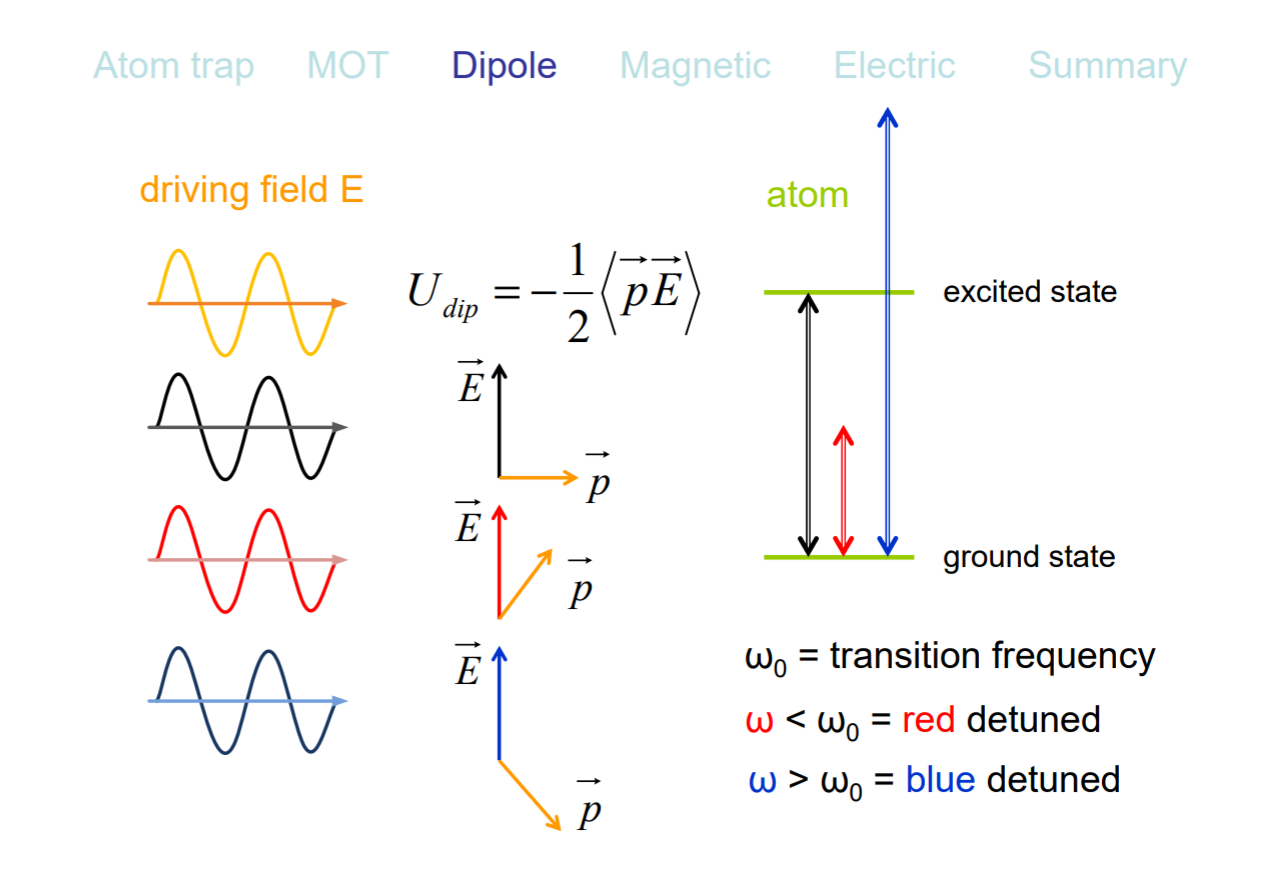
\includegraphics[scale=0.3]{slide1}
		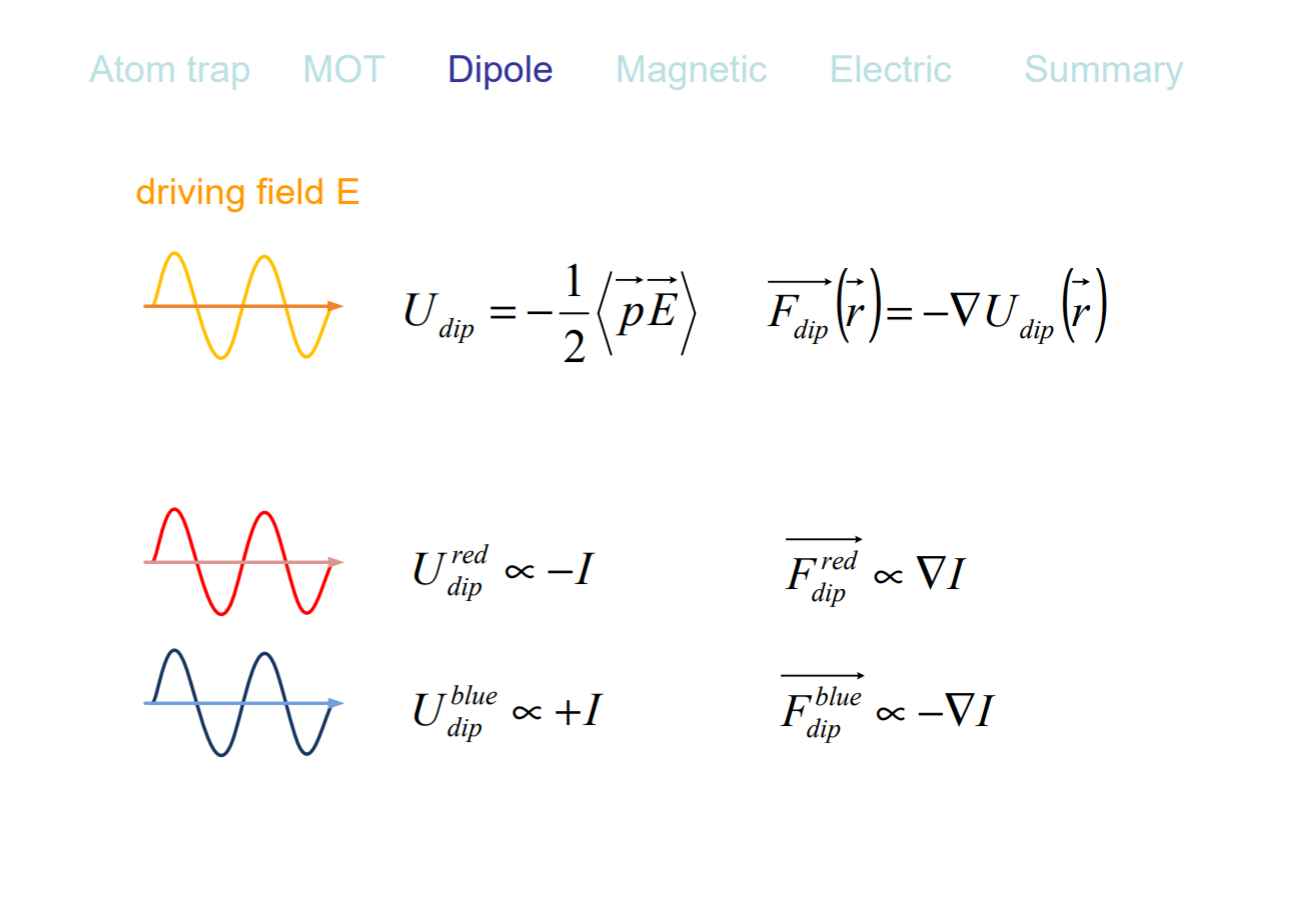
\includegraphics[scale=0.3]{slide2}
		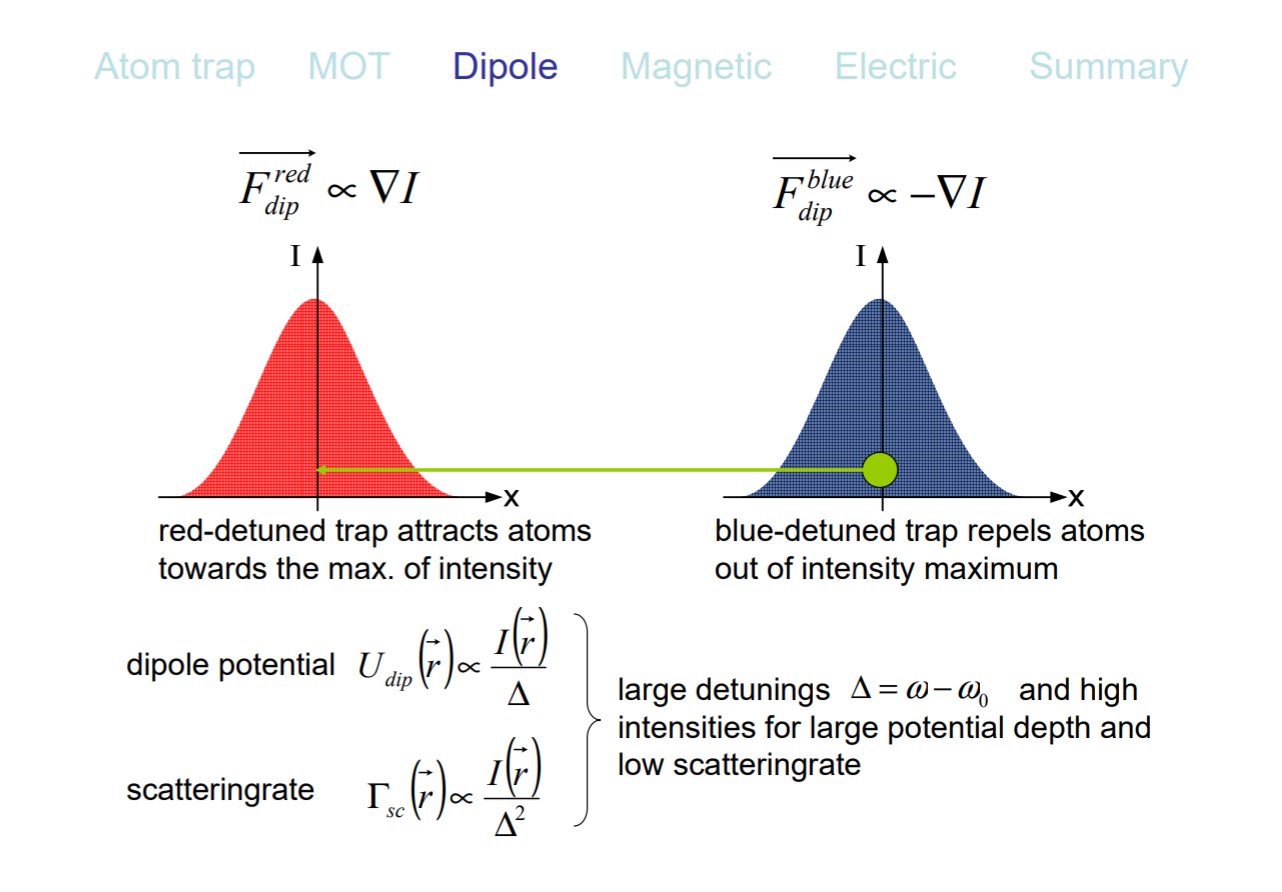
\includegraphics[scale=0.3]{slide3}
		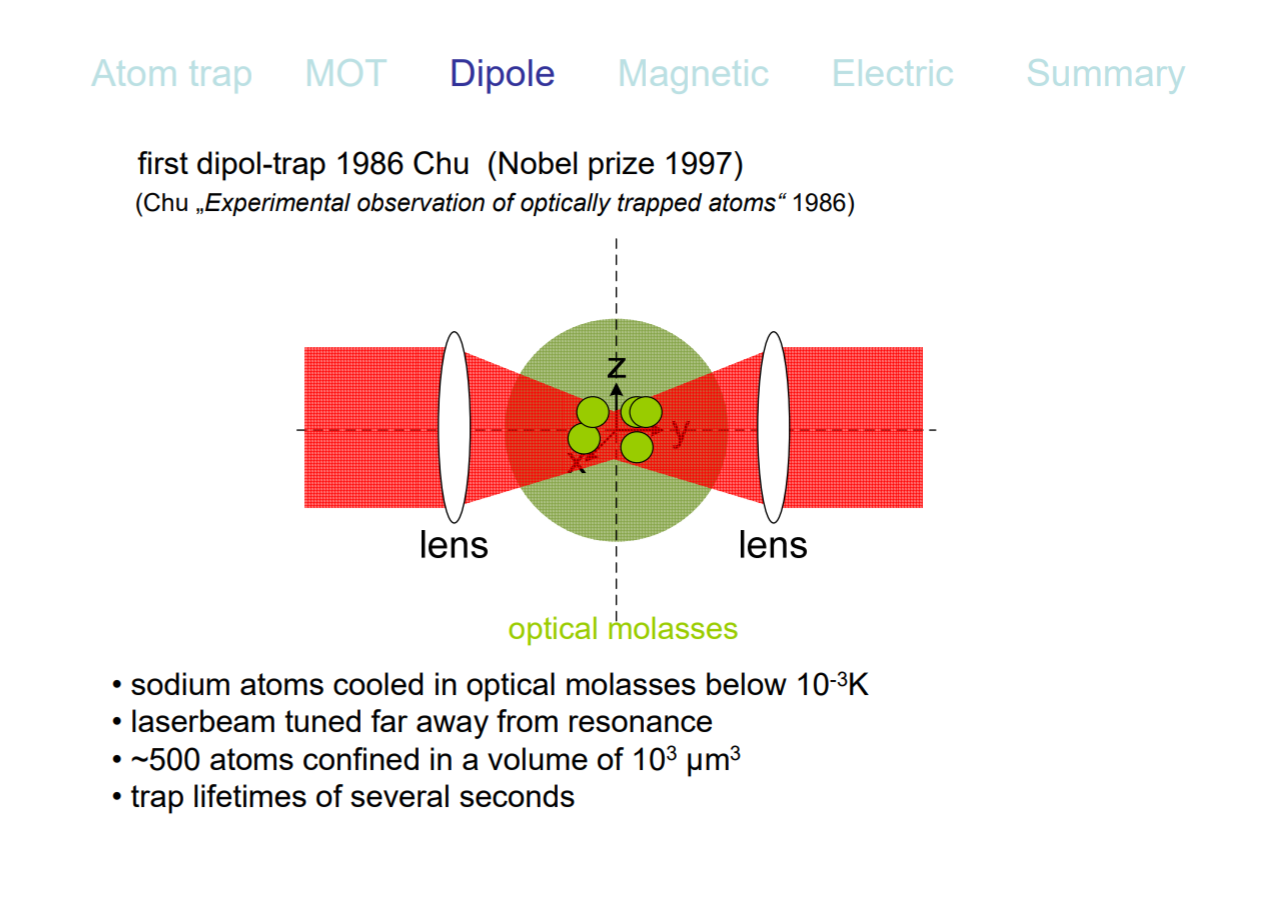
\includegraphics[scale=0.3]{slide4}
		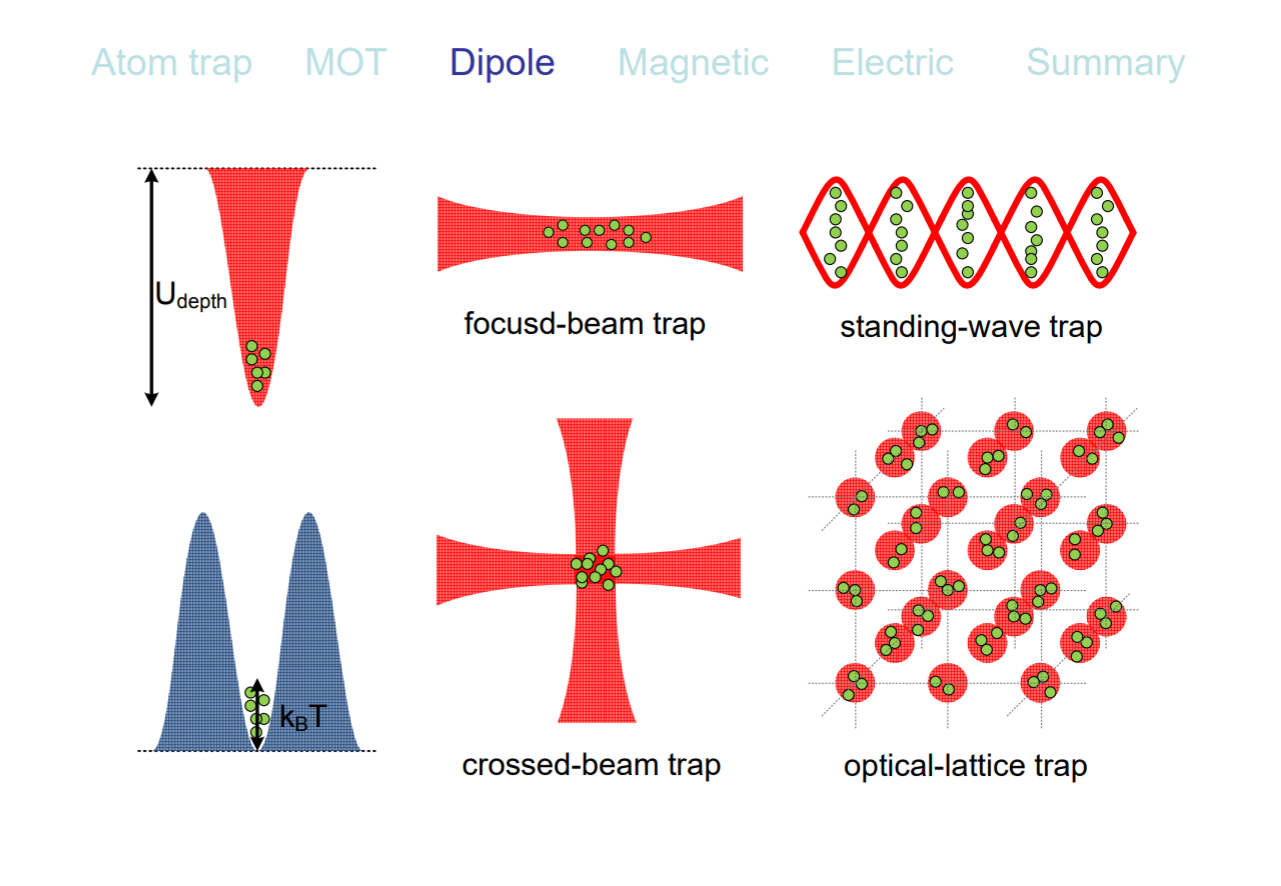
\includegraphics[scale=0.3]{slide5}
		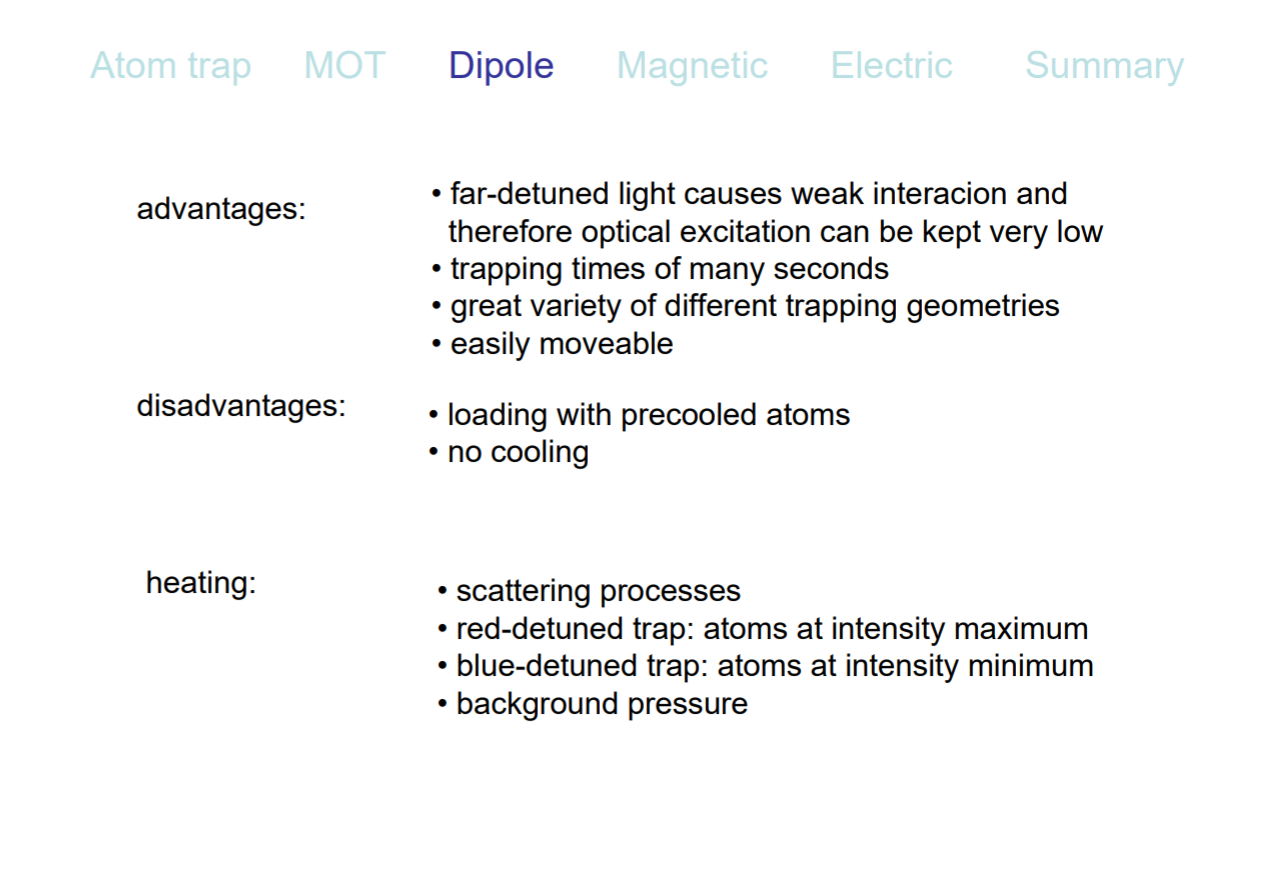
\includegraphics[scale=0.3]{slide6}
	\end{figure}
		
	\end{itemize}





\end{itemize}



\section*{Sunday, June 9, 2019}



\begin{itemize}
	\item It turns out that there are many kinds of optical dipole traps. There are red-detuned and blue-detuned, and among these are focused-beam, crossed-beam, standing-wave, and a couple of other kinds of traps. I'm interested in the standing-wave approach because of its geometry. 
	
	\item Essentially, what we want is to dipole-trap the atoms along the optical nanofiber with both red-detuned and blue-detuned methods, so as to both keep the atoms close to the nanofiber (red-detuned traps attract atoms to maximal intensity peaks) but not too close that the atoms stick to the fiber (blue-detuned traps repel atoms from the maximal intensity peaks). Explanations to any of this will eventually come as I read more, but what I can tell immediately is that the slides seem to be heavily inspired by the very same \href{https://arxiv.org/pdf/physics/9902072.pdf}{paper} I have been reading. The structure follows very well. I also see some mentioning of scaling rules, etc. This and the paper make a very good reading combination. The slides really helps with skipping the unimportant details in the paper and focusing on the main results. 
	
	\item What I now need is not only theory but what people have done to make these standing-wave traps. I managed to find a very well-written experimental \href{http://quantum-technologies.iap.uni-bonn.de/de/component/publications/?task=download\&file=69\&token=de46701d9e5eb9e185abc9784c3f8313}{paper} and a nice \href{https://www.mpq.mpg.de/5020867/0515b_atom_traps.pdf}{slideshow} that explain things pretty well. I'll make sure to take notes on the paper to actually know how to build a dipole trap. A very nice thing about that paper is that they also use the 1064 nm laser, exactly the one we will be using in Hyok's lab.
	
	
	
	\item Here's some notes on the paper by ALT et al on standing-wave dipole traps plus extra material I read on wikipedia and other sources:
	\begin{itemize}
		\item So, a standing-wave dipole trap consists of two counter-propagating Gaussian beams with equal intensities and parallel linear polarizations. Now, the paper talks about transporting the atoms, so they allow for the relative frequencies of the two counter-propagating beams to differ ($\omega$ and $\omega + \Delta \omega$) where $\Delta \omega \ll \omega$. With these, they could produce a position and time-dependent dipole potential of the form:
		\begin{align}
		V(z,\rho,t,U_0) = U_0 \f{w_0^2}{w^2(z)}e^{-2\rho^2/w^2(z)}\cos^2\lp \f{\Delta \omega}{2}t - kz \rp.
		\end{align}
		where $\lambda = c/\omega$ is the optical wavelength, $w^2 = w_0^2(1 + z^2/z_0^2)$ is the beam radius with waist $w_0$. $z_0 = \pi w_0^2 / \lambda$ is the Raleigh length. All of these quantities are shown schematically below:
		\begin{figure}[!htb]
			\centering
			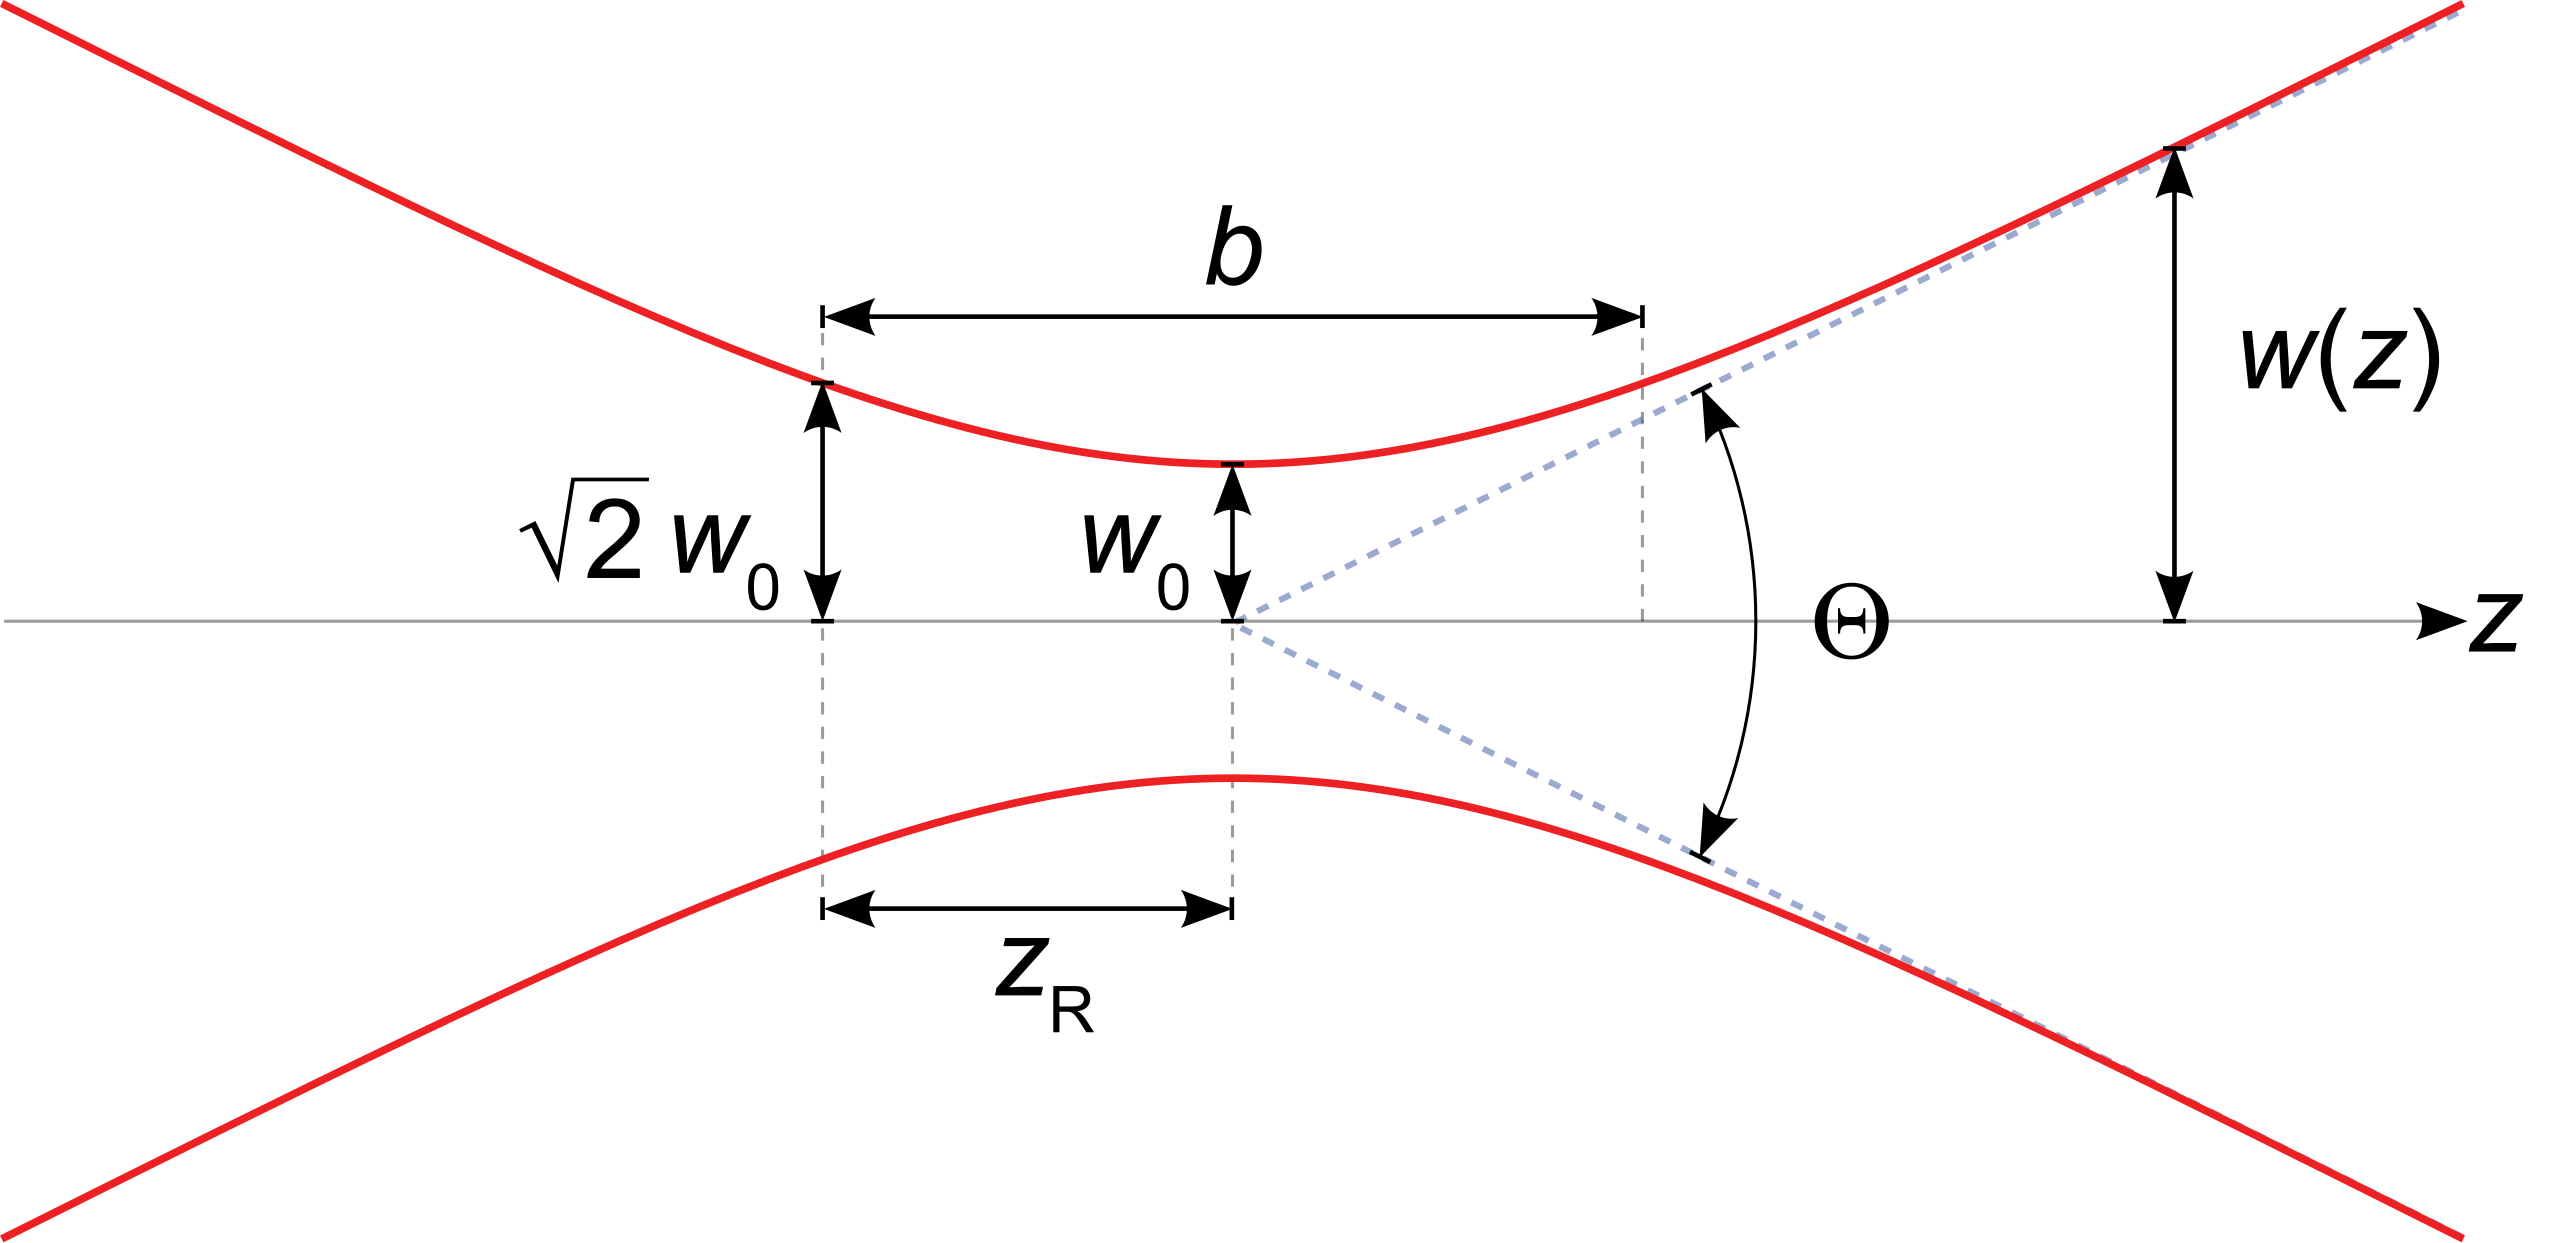
\includegraphics[scale=0.05]{gauss.png}
		\end{figure}
	
		\item Fortunately, the dipole trap used in this paper is derived from a Nd:YAG laser $\lambda = 1064$ nm, which is far red-detuned from $D_1$ and $D_2$ Cesium lines. The maximum trap depth $U_0$ is given by
		\begin{align}
		U_0 = \f{\hbar \Gamma}{2}\f{P}{\pi w_0^2 I_0}\f{\Gamma}{\Delta}.
		\end{align}
		$\Gamma = 2\pi \times \omega'$ is the natural linewidth of some transition. $I_0$ is the corresponding saturation intensity. $P$ is the total power of both laser beams. For red-detunings, $\Delta < 0$, the dipole potential provides a three-dimensional confinement with a trap depth of $\abs{U_0}$. For alkalies, the effective detuning $\Delta$ is given by
		\begin{align}
		\f{1}{\Delta} = \f{1}{3}\lp \f{1}{\Delta_1} + \f{2}{\Delta_2} \rp
		\end{align}
		where $\Delta_i$ is the detuning from the $D_i$ line. With the rest of the parameters known, we can calculate the potential depth $U_0$ in Kelvin.
		 
		\begin{figure}[!htb]
			\centering
			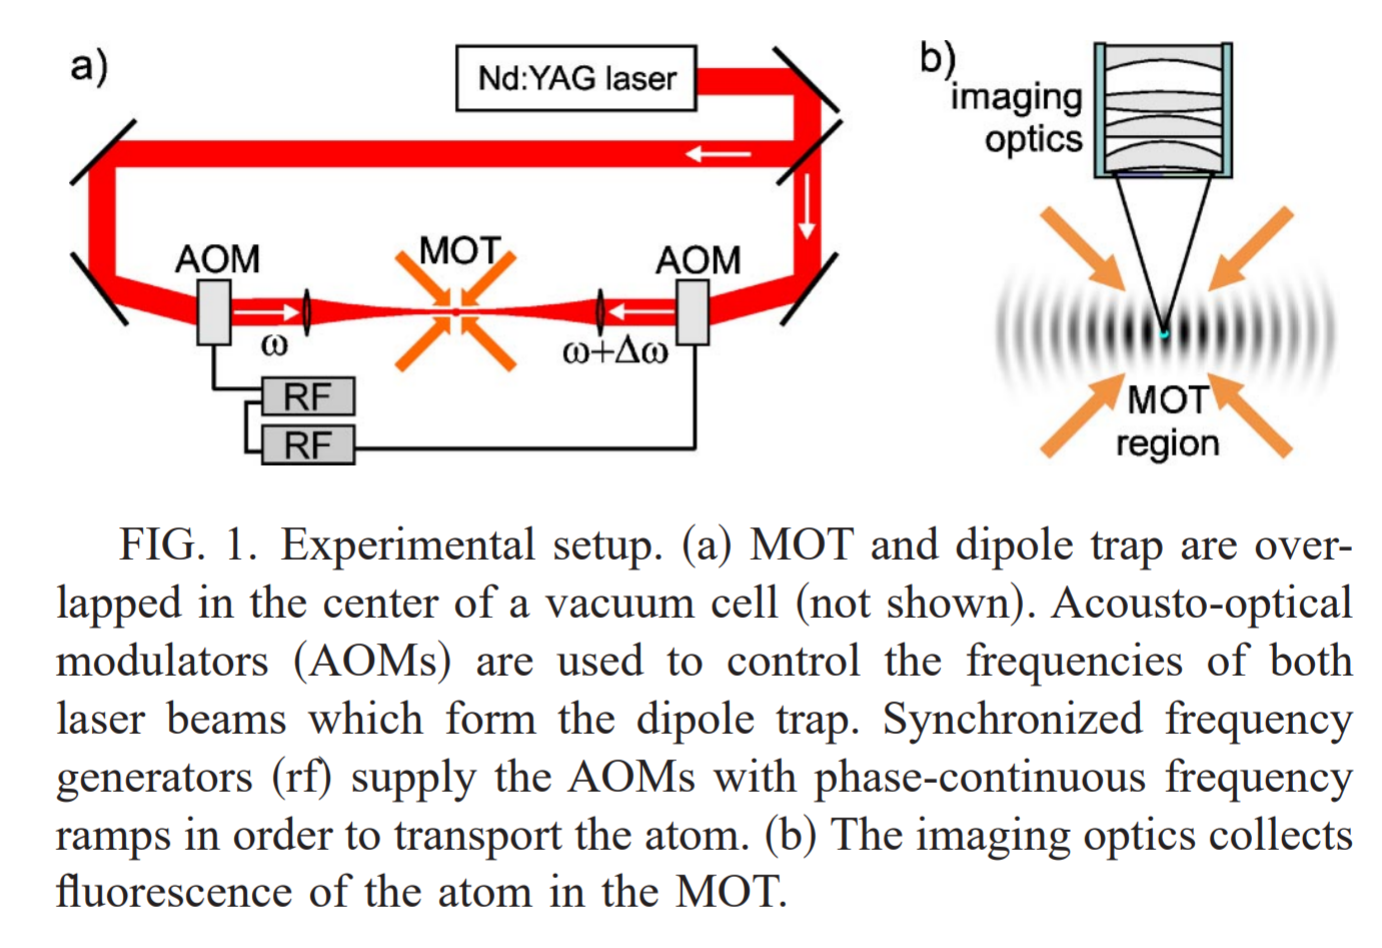
\includegraphics[scale=0.5]{dipole.png}
		\end{figure}
	
	
		\item An atom of mass $m$ trapped in such a standing-wave potential oscillates (in harmonic approximation) with frequencies
		\begin{align}
		&\Omega_z = 2\pi \sqrt{\f{2U_0}{m\lambda^2}},\\
		&\Omega_\text{rad} = \sqrt{\f{4U_0}{mw_0^2}}.
		\end{align}
		If we know the mass of the atoms and beam waist $w_0$ and other beam parameters we can find these frequencies.
		
 	\end{itemize}
 
 
 
 	\item I also found an excellent \href{https://www.phas.ubc.ca/~qdg/publications/GraduateTheses/thesis_hon_Gao.pdf}{paper} by a student from the University of British Columbia on building a standing-wave optical dipole trap. This is an almost-perfect combination of theory and experiments. From a quick read-through I found that a lot of the theory came from Grimm's \href{https://arxiv.org/pdf/physics/9902072.pdf}{paper}, which is a good thing for me as I'm sure the new knowledge from this paper is consistent with what I have read before. The experimental procedures are also very well laid out. This paper is probably something I can refer to when I run into trouble. The paper also seems to be using some kind of combination of Python and LabView - which is pretty good considering my plans for building a dipole trap and moving the lab from LabView to Python.
\end{itemize}





\chapter{Bureaucratic Limbo}

\section*{Monday, June 10, 2019}

\begin{itemize}
	\item I'm back on UMD campus, still waiting for my OPT application to get approved. If it doesn't get approved soon, I won't get my EAD card this week, which means I'll lose another week of the program.
	
	
	\item It's the end of the day. I heard nothing. Three people from Colby have gotten their OPT approved so far. One got approved today. I hate to say this but I'm losing hope I'm getting anything by the end of this week. 
	
	
	\item I can't do any work in this kind of limbo. I'd rather be out of a job, or not having a job at all, than being stuck in this indeterminate state. Will the EAD come? It might. OK. But when? This week? A week from now? Two weeks from now? When I'm on the plane back home? Can I even BE on a plane back home while my application is still processing?

	
	\item I emailed Hyok this morning for more resources on the two-color optical dipole trap. It turned out that both Grover and Solan somewhat mentioned how to implement this in their papers. I will take notes on these in the near future. 
	
	\item Solano's ONF \href{https://arxiv.org/pdf/1703.10533.pdf}{review} on the arXiv, page 28. 
	
	\item Grover's \href{https://drum.lib.umd.edu/handle/1903/16638}{thesis}, Chapter 3. 
	
	\item If these link are broken, these papers can be found on my GitHub repository. 

\end{itemize}



\section*{Tuesday, June 11, 2019}

\begin{itemize}
	\item No updates on the OPT case. 
	
	
	\item \textit{Grover's thesis, chapter 3:} N/A
	
	
	\item \textit{Solano's ONF review, page 28:} N/A
	
	\item Hyok sent me a link to a nice seminar at JQI a few years ago. Here's the \href{https://www.youtube.com/watch?v=IFsB554TCZY}{link} to the talk. It was good, and I learned something.
	
	\item I failed to read the articles I intended to read today. For me the whole OPT situation is going to be decided this week, in a not-too-good or bad way. I've already lost a big chunk of my time here, and I'm pretty sure I'm not going to have enough time to work on translating LabView to Python. I don't even know if I have enough time for the dipole trap. 
	
	\item To get anything done in this short amount of time I might have to work over time. I don't mind this. I'm willing to work late and on weekends. It's possible. The only problem right now is a piece of plastic that should have been in the mail 10 days ago.
	
	\item Is this part of what being an international student is like? I certainly feel cheated by the administrative people who are and/or should be involved in all this work permit application mess. I couldn't apply more than 90 days from the start date, yet it's already taking them 90 days and counting to process the damn case. 
	
	\item It's Wednesday tomorrow. There's going to be a lab group meeting. But I don't think I'll be there as I don't think I can call myself a group member with 2 days in the lab.
	
	\item There's going to be a JQI seminar on Thursday which I plan to attend. 
	
	
\end{itemize}



\section*{Thursday, June 12, 2019}
\begin{itemize}
	\item Still no progress on the papers I was planning to read.
	
	\item I went to the conference room but decided against attending it. I called USCIS instead to check the status of my case. It turned out that they have rejected my request to expedite the case a long time ago without noticing me. This means the congresswoman wasn't very helpful.
\end{itemize}

\chapter{The wait ends}
\section*{Wednesday, June 19, 2019}
\begin{itemize}
	\item Not much happened between the last time I updated the journal and today. I read a bit and updated my QM notes. I still haven't started on the papers I was {supposed} to be reading.
	
	\item The desperate wait finally ended when at 4:00 PM today I received a text message saying there was an update on my case. When I came and checked the status online it said my EAD card was being produced. This means the case was finally approved, and that I can start working next week when the card arrives.
	
\end{itemize}

\section*{Friday, June 21, 2019}
\begin{itemize}
	\item I attended a lab meeting for the first time. It was a brainstorming session between experimentalists and theorists. While I couldn't appreciate a lot of the technical details, I was able to grasp what a typically brainstorming session is like here. It was clear that there were Steve Rolston, who was like the ``chief'' of the experimentalists (which included me), Alexei, the ``chief'' of the theorists, and Kanupriya, who seems to be in charge of the theory related directly to the nanofiber experiment we're working on. 
\end{itemize}

\section*{Saturday, June 22, 2019}
\begin{itemize}
	\item It's a good time now to reboot my system and get ready to actually go to the lab and implement the optical dipole trap. This means I'll absolutely have to finish reading the papers and at least understand how it works. I would assume this won't take too long. I just need to get started...
	
	\item On another note, I sent two emails today, one to Hyok to discuss the next steps and one to Kanu to ask for theory material on the nanofiber experiment. There was a lot of talk about sub-radiance, super-radiance, super-duper-radiance, and so on, related to the nanofiber experiment that I want to have a look at. 
	
	\item \textbf{What are evanescent fields?} To answer this question, we look at the phenomenon of \textit{total internal reflection}. 
	
	\begin{itemize}
		\item We first look at Snell's law:
		\begin{figure}[!htb]
			\centering
			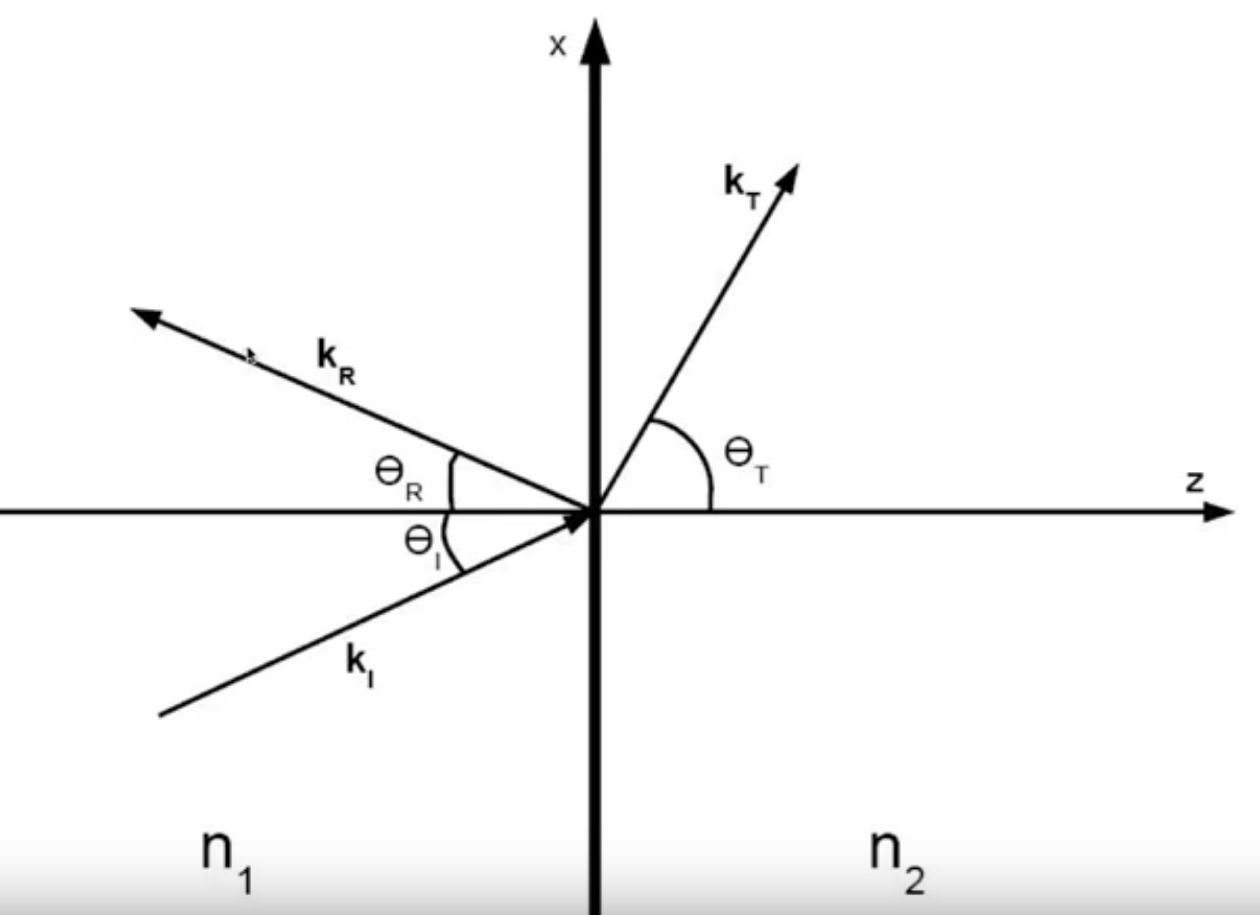
\includegraphics[scale=0.3]{snells-law}
		\end{figure}
	
		Snell's law says that
		\begin{align}
		n_1\sin\theta_I= n_2\sin\theta_T
		\end{align}
		where $n_i$ is the index of refraction in the medium $i$. From this, we have
		\begin{align}
		\theta_T = \sin^{-1}\lp \f{n_1}{n_2}\sin\theta_I \rp. 
		\end{align}
		Because $\sin\theta_T$ cannot be greater than 1, we define 
		\begin{align}
		\theta_C = \sin^{-1}\f{n_2}{n_1}
		\end{align}
		to be the critical angle (above which ($\theta_I > \theta_C$) we get ``total'' internal reflection). Total internal reflection is a phenomenon when light incident on surface completely reflects off of it back into the medium from which it came. 
		
		\item What we are interested in now is what happens when $\theta_I > \theta_C$, or when ``$\sin\theta_T > 1$.'' Let us express the electric field associated with the emitted light as
		\begin{align}
		\vec{E}_T = \vec{E}_{0T}e^{i(\vec{K}\cdot\vec{\gamma} - \omega t)}
		\end{align}
		where $\vec{E}_{0T}$ denotes the amplitude vector and $\gamma$ is the position (or propagation) vector. Now, we know that
		\begin{align}
		\vec{K}\cdot\vec{\gamma} = k_x x + k_y y + k_z z = k_x x + k_z z 
		\end{align}
		because there's no propagation component in the $y$ axis. We also have that
		\begin{align}
		&k_x = k_T \sin\theta_T\\
		&k_z = k_T \cos\theta_T
		\end{align}
		so,
		\begin{align}
		\vec{E}_T = \vec{E}_{0T}e^{-\omega t}e^{i(k_T\sin\theta_T)x}e^{i(k_T\cos\theta_T)z}.
		\end{align}
		Now, we know that because $\theta_I > \theta_C$, $\sin\theta_T > 1$. This means $\cos\theta_T$ must be imaginary, because $\sin^2\theta_T + \cos^2\theta_T = 1$. And because $k_T$ is real, we must have
		\begin{align}
		k_T\cos\theta_T = Ai
		\end{align}
		where $A$ is some real factor. Thus,
		\begin{align}
		\vec{E}_T = \lp\vec{E}_{0T}e^{-\omega t}e^{i(k_T\sin\theta_T)x}\rp e^{-Az}.
		\end{align}
		Because we're only interested in the real part of the electric field, 
		\begin{align}
		\boxed{\Re{\vec{E}_{T}} = \vec{E}_{0T}\cos\lb (k_T\sin\theta_T)x - \omega t \rb e^{-Az}}
		\end{align}
		This describes an ``evanescent'' field, as it decays exponentially from the surface in the $+z$ direction. 
		\begin{figure}[!htb]
			\centering
			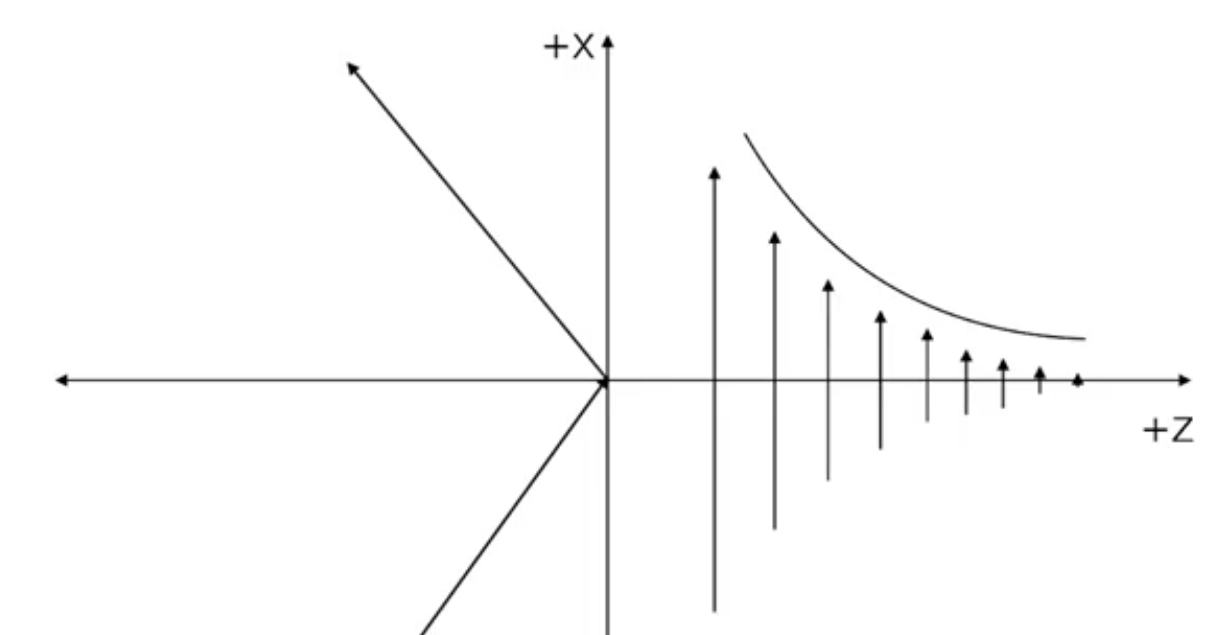
\includegraphics[scale=0.5]{evanes}
		\end{figure}
	
	\item We note that evanescent waves don't propagate as an EM wave. Its energy is concentrated spatially in the vicinity of the source - the boundary of the material. There is no net energy flow. The Poynting vector when averaged algebraically over a complete oscillation results in zero. The physical explanation for the existence of the evanescent waves is that the electric and magnetic fields cannot be discontinuous at a boundary.
	
	
	\item Here is some nice graphics from Wikipedia:
	\begin{figure}[!htb]
		\centering
		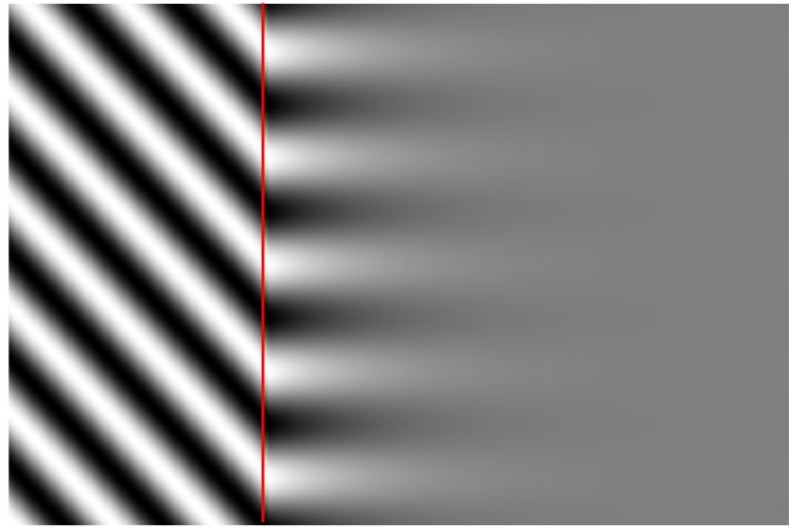
\includegraphics[scale=0.7]{evanes-wiki}
	\end{figure}
	\end{itemize}
	
	
	\item \textbf{Solano's ONF review, page 28:} This section in the paper is called ``\textit{Trapping atoms around on optical nanofiber.}'' So we have seen how free space beams can be used to generate a dipole trap. It turns out that evanescent fields from an ONF can also do the trick. Solano's ONF review gives an overview of the \textit{setup} of the dipole trap being used with their then ONF at JQI, and the \textit{confirmation} that the trap actually worked. 
	
	\begin{itemize}
		\item \textbf{Setup:} The  ONF has waist diameter $500 \pm 50$ nm with length of 7 mm and 28 mm tapering region. MOT species was Rb, cloud of $10^8$ atoms. The cloud is overlapped with the ONF, using shim coils and UHV manipulator. 
		
		\item Two lasers were needed for this particular dipole trap: red- (1064 nm) and blue-detuned (750 nm). The red-detuned laser creates an attractive potential, while the blue prevents the atoms from striking the ONF. A potential minimum is formed at $\sim$ 200 nm from the fiber surface, based on calculation with \textit{two-level atoms} and \textit{scalar shift}. The blue-detuned beam and probe beam (780 nm) are intensity-stabilized. 
		
		\item We might have to worry about polarizations, but I won't go into that for now.
		
		\item Attached here is the schematics:
		\begin{figure}[!htb]
			\centering
			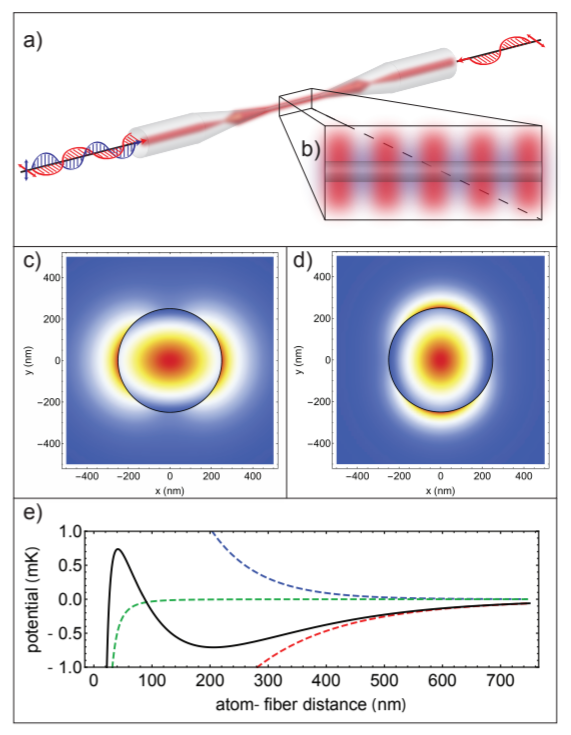
\includegraphics[scale=0.9]{dipole-trap}
		\end{figure}
	
	
		\item (a) The 1064 nm beam is put in a standing-wave configuration, linearly polarized. The 750 nm beam is orthogonally-polarized compared to the red beam. (b)  Illustration of potential at the
		ONF waist with lattice formed by 1064-nm beams. (c) Intensity plot of 1 mW of linearly-polarized, 1064-nm light in an ONF with diameter 500 nm. The color scale indicates increasing intensity from blue to red. (d) Intensity profile of vertically-polarized 750-nm light through the same ONF. (e) Total trapping potential (black) for a 500-nm diameter ONF
		with contributions from 3 mW in each 1064-nm beam (red dashed), 6.5
		mW of 750-nm power (blue dashed), and van der Waals (green dashed).
		The potentials are calculated from only the scalar shifts. 
		
		\item The counter-propagating red beams create two 1-D optical lattices. 
	\end{itemize} 



	\item \textbf{Grover's thesis, Chapter 3:} The system used in Grover's thesis the same as that in Solano's review. This thesis gives more technical details regarding the implementation of the trap. 
	
	\begin{itemize}
		\item Attached here is the setup of the dipole trap:
		\begin{figure}[!htb]
			\centering
			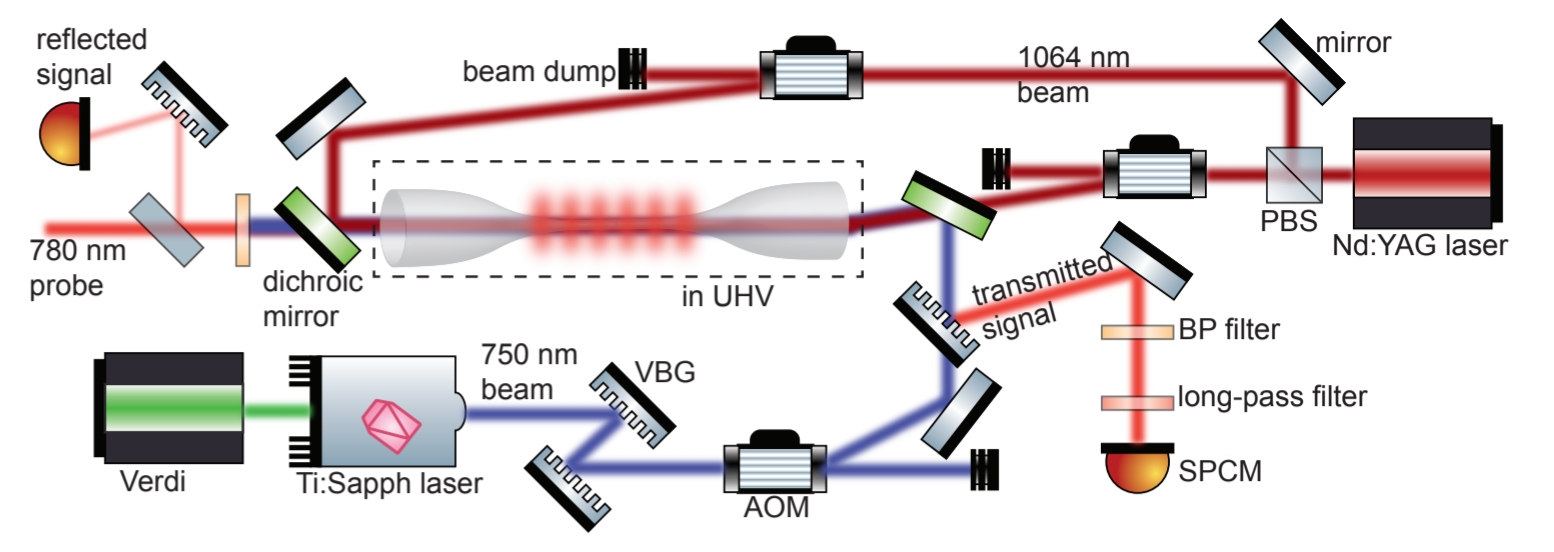
\includegraphics[scale=0.5]{dipole-trap-setup}
		\end{figure}
	
	
		\item  Experimental schematic. Beams from the Nd:YAG laser (1064 nm)
		and the Ti:Sapph laser (750 nm) are coupled onto the nanofiber using dichroic mirrors. Thru-fiber absorption signals are measured with SPCMs. Volume Bragg gratings (VBGs) o↵er narrow-line filtering of spurious background the Ti:Sapph laser as well as fluorescence from impurities in the fiber glass. See text for details.
	\end{itemize}
\end{itemize}


\chapter{Reboot}
\section*{Tuesday, June 25, 2019}
\begin{itemize}
	\item I met Kanupriya, our group's theorist. We talked for about an hour and a half about some of the theory behind the phenomena in the experiment. She gave me some book recommendations and some topics to look into in quantum mechanics including the density operator, deriving spontaneous emission, and ultimately sub- and super-radiance. It was a very helpful discussion, for now I have a better idea of what texts to look into for the theory involved in the experiments. 
	
	\item I got a bike from craigslist. It's a Japanese-made Iverson, probably from the late-70s or 80s. The dealer's name was Gil. Bike enthusiast. We chatted a little bit about bikes and other things. I think the bike was a great buy for 130 bucks. It's not easy to find a decent bike for less than 200 in the US I'm sure. I like the geometry of the frame and the vintage look. The frame is of course stainless steel. Very comfortable ride (although that means power transfer is abysmal). The components are probably as old as the bike is. I'll eventually swap them out for more modern pieces. The handlebar is quite short, definitely shorter than the already narrow 42 cm. It'll take a few rides before I can be confident on the saddle.   
\end{itemize}

\section*{Wednesday, June 26, 2019}
\begin{itemize}
	\item I met professor Dennis Papadopoulos today. He's a professor of plasma space physics here at UMD. He's a friend of a friend of my aunt. There's no particular reason why my aunt and her friend want to put me in contact with him, but it was delightful to meet and talk to him nevertheless. He's in his 80s now but still quite active in research. He works with these antennas that send currents into space to study the dynamics of radiation around Earth. I don't know much about this stuff but it sounds interesting and obviously very sophisticated. 
\end{itemize}


\end{document}
